Cloud systems have gained popularity over the last decade by enabling users to store data, host
applications and perform computations over the network. Cloud systems significantly decrease
the cost on the user end as management, maintenance and administration tasks are typically
handled by the cloud providers. Cloud providers also benefit from this scheme as they can
utilize system resources more efficiently through techniques, such as virtualization, enabling them
to achieve better performance and energy efficiency. There are numerous cloud providers
offering a broad range of services~\cite{googlece, aws, azure}.

Even though cloud systems tend to have lower energy costs compared to traditional HPC clusters
due to better utilization techniques, the increasing energy consumption of cloud systems still
needs to be addressed as the amount of data stored and the number of computations and applications
in cloud increase steadily. According to \cite{Kaushik:2010:LSE:1851476.1851523}, the estimated
energy consumption of U.S. data centers was more than 100 billion Kilowatt hours in 2011.
Between 2005 and 2010, data centers consumed between 1.7\% and 2.2\% of all electricity in the
U.S.~\cite{koomey2011growth}, matching the energy consumption of the aviation industry.
Increasing energy consumption also means higher cooling costs and additionally, a cloud system with an
underperforming cooling mechanism may have reliability issues potentially causing violations of
service-level agreements (SLA) with the cloud users. It is, therefore, very important to have an
energy-efficient cloud system not only for lower energy costs, but to also meet performance
demands of the cloud users as well.

A typical cloud system is shown in Figure~\ref{fig:cloud_architecture}. In this work, we refer to any 
application using the backend storage of a cloud system as the \textit{user} of that storage system.
There are several components in a cloud system contributing to the overall energy consumption - namely
 processing units, network
components and storage systems. In this work, we specifically target the energy consumption of the
cloud storage infrastructure forming the backend of the cloud computing units, since the storage
system costs constitute an important fraction (between 25-35\%) of overall cloud system
costs~\cite{Harnik:2009:LPM:1586640.1587438, Kim:2011:EPD:1951365.1951378, netapp_power}. Storage
systems also have more idle periods since data stored is usually redundant and archival, written once
and not touched again~\cite{Miller93}. There have been many studies to reduce the energy consumption of
other components of cloud systems. However, since idleness is not usually available in the network
and processing units of clouds, these studies have been mostly on virtual machine consolidation,
workload characterization, data migration or scheduling. In this work, we propose methods to have
an energy-aware cloud storage system while at the same time trying to achieve uniform system
utilization on demand. In particular, we take advantage of idleness existing in cloud storage systems
and try to switch inactive nodes into low power modes. Our work is driven by two key assumptions: first,
the cloud storage system suffers from incasting, and second, most of the data stored in the cloud (as much
as 75\%) is not heavily accessed~\cite{netapp_power}, creating idle periods. It is
important to note that our methods can also be implemented in the storage systems that form the backend
of computational platforms (i.e. Hadoop clusters), where there might be idle
periods~\cite{Kaushik:2010:GTE:1924920.1924927, Narayanan:2008:WOP:1416944.1416949}.


\begin{figure}[!htbp]
\centering
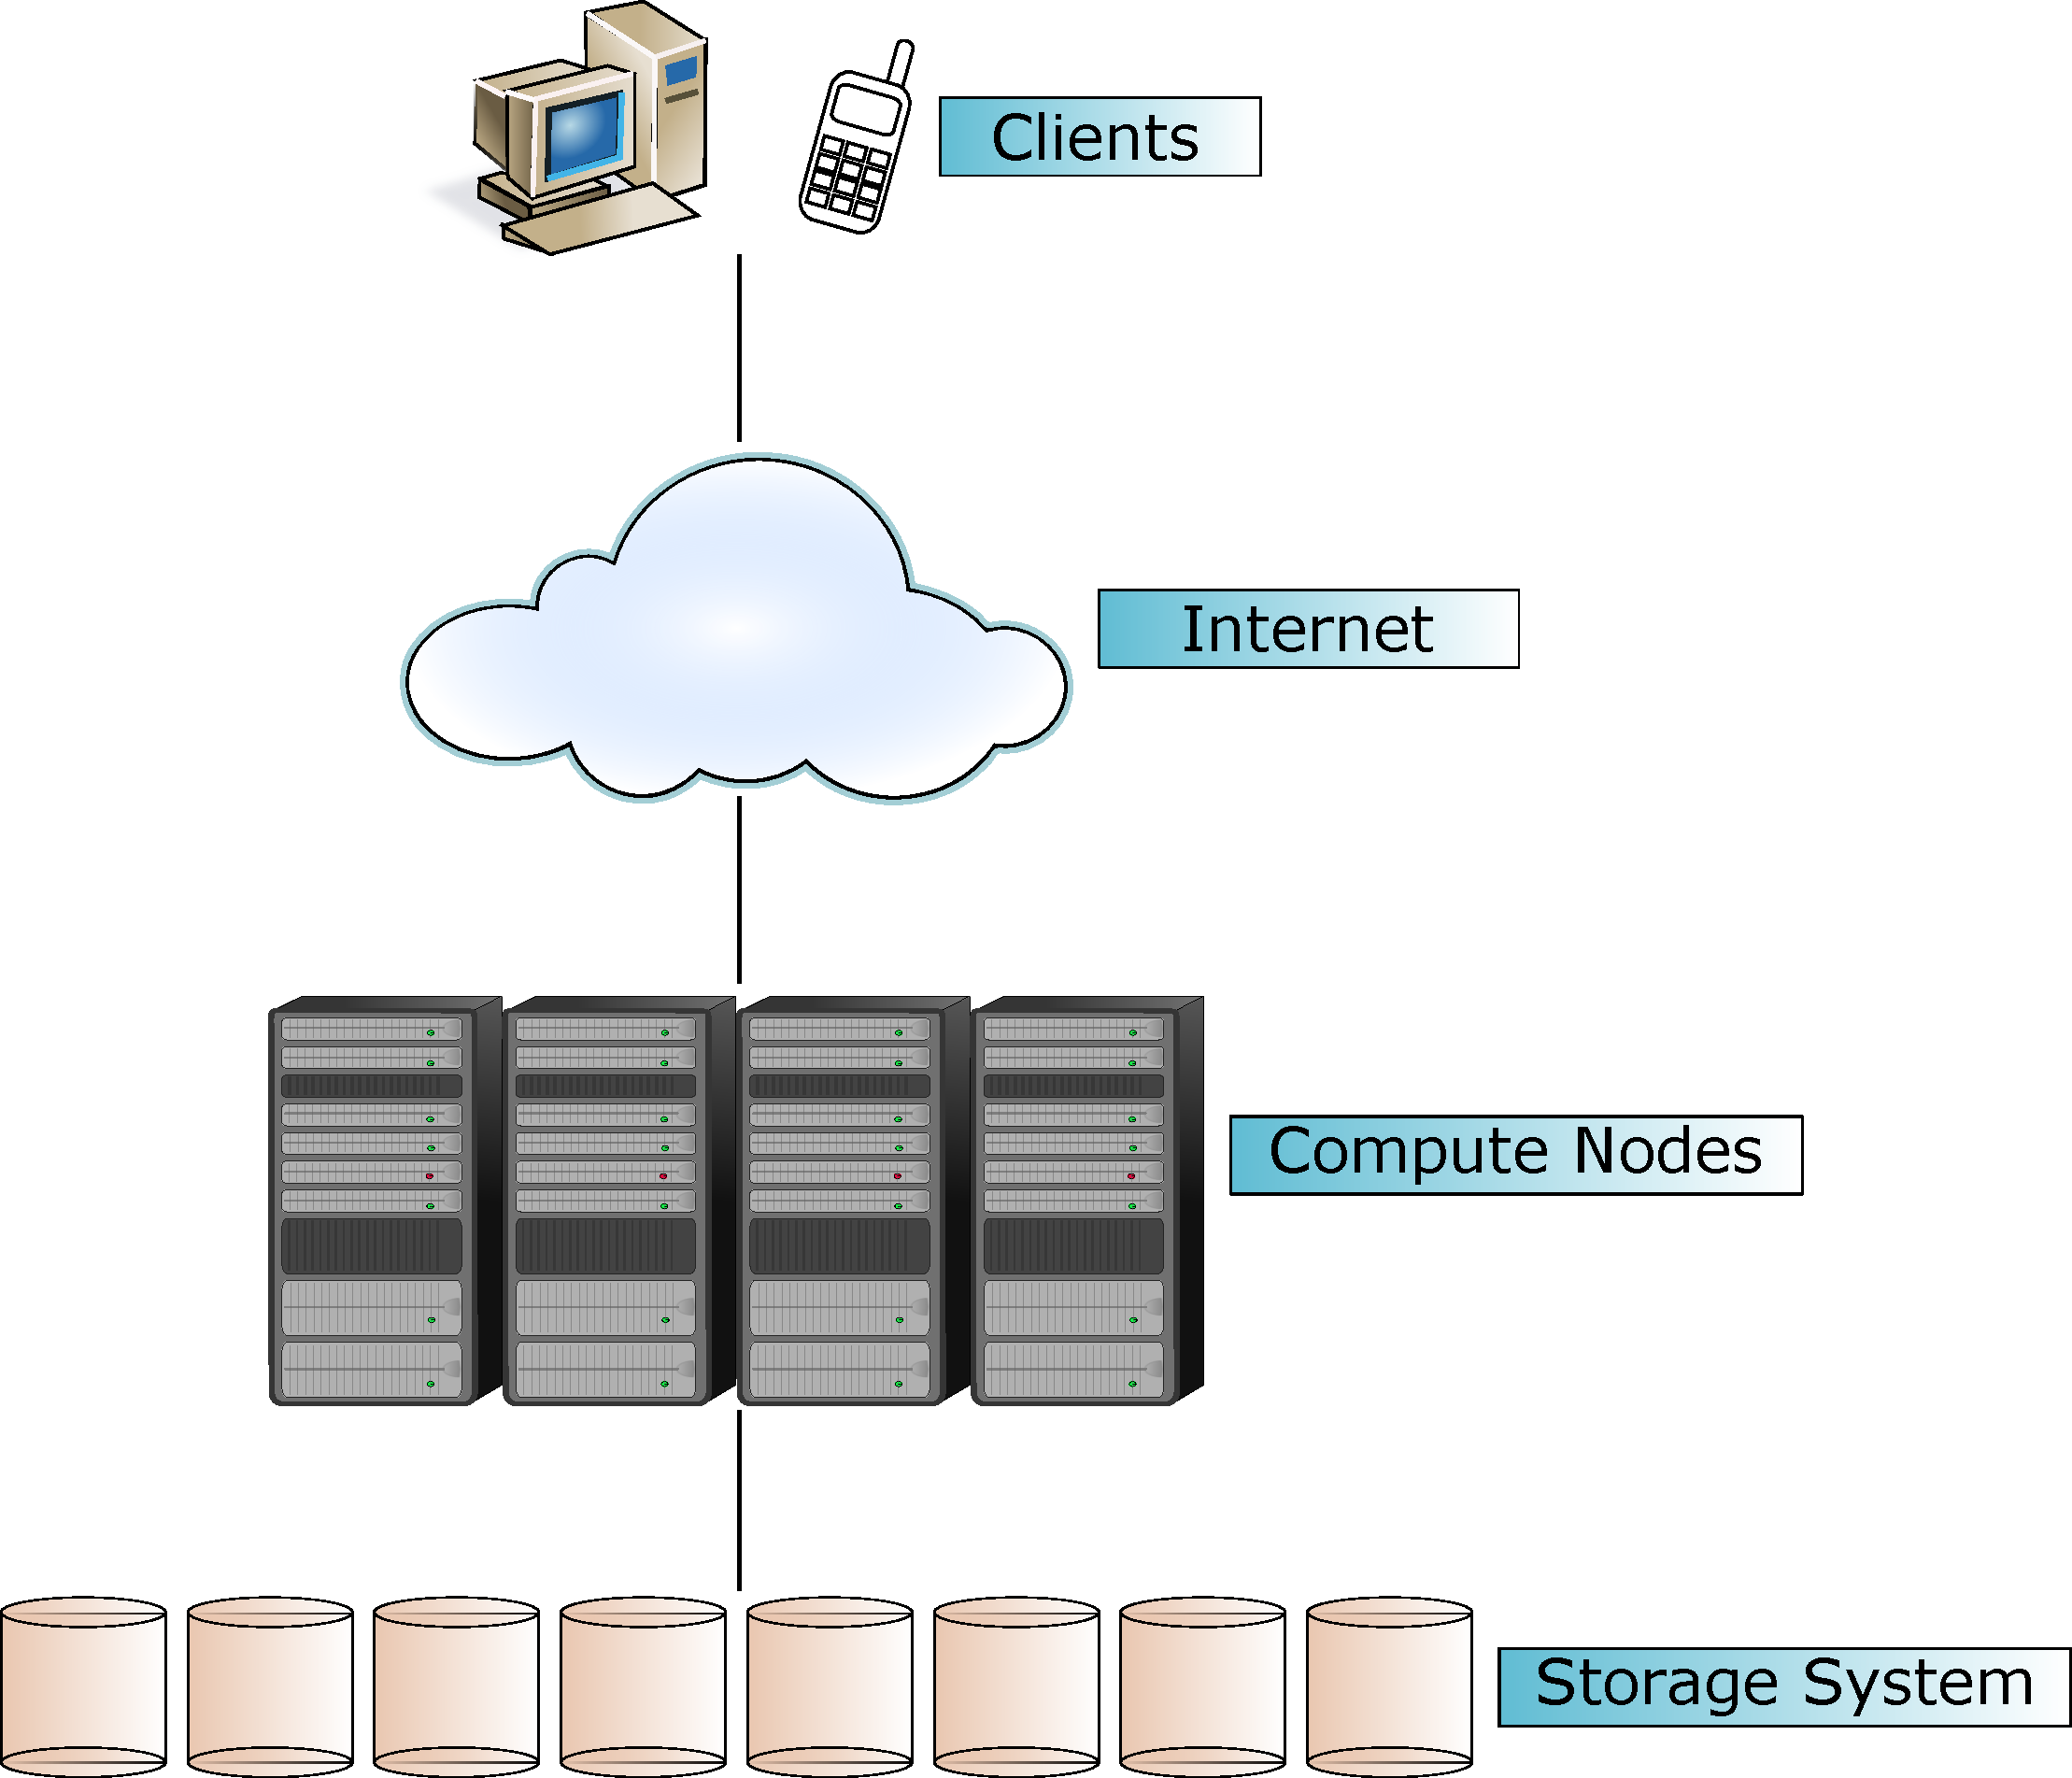
\includegraphics[width=\columnwidth,keepaspectratio]{FIG1.pdf}
\caption{Typical cloud system architecture}
\label{fig:cloud_architecture}
\end{figure}

% XXX Before talking about incasting explain the traditional structure
% XXX of a parallel storage system - e.g. a SAN with parallel storage
% XXX nodes connected through a switch with cloud compute nodes.  A
% XXX reference to the earlier figure might be useful
\textit{Incasting} is a condition that occurs because of queue limitations in most network
switches~\cite{Nagle:2004:PAS:1048933.1049998}. As a result of the incasting behavior, there
is a limit to the number of storage nodes (e.g. 4 servers in a cluster-based storage network
as in~\cite{Krevat:2007:AAA:1374596.1374598}) across which data can be
striped for parallel access. Beyond this limit,
the I/O bandwidth no longer scales and in fact deteriorates. If $M$ represents the number of nodes at
which the performance maxes out, from a performance point of view, there is no point in using more
than $M$ nodes to increase parallelism. While for performance scaling, we would only need $M$ storage nodes in the system,
however, for storage capacity reasons, we may need more than $M$ nodes. In such systems, we would
need to keep these extra nodes active and thus waste energy since the network resources are maxed-out
by a \textit{subset} (of size $M$) of the storage nodes.

To save energy, one could turn off these extra storage nodes, and activate them when necessary. The
difficulty comes while trying to identify which storage nodes should be turned on or off. Our approach
is to distribute cloud users across the storage nodes, such that each user is allocated only $M$
nodes - i.e. the limit at which performance is maxed out. Grouping data on a subset of the storage nodes
and putting the remaining nodes into low power modes has been studied in many related
studies~\cite{Kaushik:2010:GTE:1924920.1924927, Kaushik:2010:LSE:1851476.1851523, Leverich:2010:EEH:1740390.1740405}.
However, the majority of these studies used data classifications,
redundant data or a hot-cold zone approach
to group data on a subset of the storage nodes. Our approach is different from existing studies in that
we try to group \textit{cloud users} on a subset of the storage nodes without any data classification. Not
classifying data enables our methods to be implemented in cloud storage systems with any kind of
redundancy scheme. It is important to also note that, because of the job processing structure (batch mode or
intelligent schedulers) in clouds, we can effectively turn on and off storage nodes based on the user job
submissions since we know a priori which $M$ nodes are going to be used at any time. Therefore, any latency
due to transitioning a storage node from inactive to active mode can be hidden. 

The challenge becomes now how to allocate a subset of cloud storage nodes for each user in order to reduce 
the energy footprint, while at the same time trying to preserve uniform distribution of the system resources if
demanded. We exploit the heterogeneity in the user metadata for energy-aware storage node allocation. As an
example, if we assume a storage system consists of $N$ storage nodes and $M$ of them
max out the incast bandwidth ($N > M$), then each user can be assigned a separate subset of $M$ storage
nodes based on a certain metadata (i.e. user id, usage pattern) and any storage node that is not allocated
for any user at that time can be switched into a low power mode. In this paper, we present several methods
to map subsets of storage nodes to different cloud users and show their outcomes with extensive simulations
using real-world workloads. These approaches build extensively on preliminary methods we presented in our
earlier work~\cite{6322247}.

The rest of this paper is organized as follows: 
Section~\ref{related} gives a brief overview of the related studies. 
Section~\ref{methods} describes the implementation of the node allocation methods we are proposing.
Section~\ref{model} presents a mathematical model to estimate the outcomes of the proposed methods.
Section~\ref{theory} evaluates the proposed methods theoretically to show their approximation factors
to the optimal solutions.
Section~\ref{results} gives the experimental evaluation results of the proposed node allocation methods
and validates the mathematical model proposed in Section~\ref{model}.
Finally, we present conclusions and possible future work in Section~\ref{conclusion}.
